\chapter{Related Work}

In the following section, we investigate the current state of research on 6D pose estimation. The chapter starts with an excerpt of non-learning-based methods. We then present the latest papers and analyze publications on active learning and fine-tuning of neural networks.

\section{Research on 6D Pose Estimation}

Pose estimation has become an increasingly interesting problem with the advent of robots in production and the area of virtual and augmented reality \cite{bb8}. Research before the rise of learning-based methods focused on manual feature extraction, divided into the major groups of sparse, dense and template-based approaches. Nowadays scientists often employ learning-based techniques which offer higher accuracy.

\subsection{Non-Learning-Based}

Before the major breakthrough of deep learning in 2012 \cite{alexnet}, handcrafted feature-based approaches were common for 6D pose estimation \cite{ylecun}. A lot of research \cite{gklein,dglowe2,charris} makes use of edges to detect 3D objects, but were therefore sensitive to occlusion. Methods relying on keypoints \cite{dglowe1, dwagner} work well on well-textured objects. But they yield bad performance on poor-textured or texture-less objects, due to detectors find unstable keypoints or none at all. 
\nnewline
An intuitive idea to improve the quality of the estimate is to use stereo cameras, as implemented in \cite{kpauwels}. A second image from another angle provides depth information to a certain extend but involes the additional task of stereo matching. The sudden availability of cheap depth sensors, like the Kinect, gave rise to algorithms making use of RGB-D images. Different approaches are possible when incorporating depth to retrieve an object's pose. \cite{bdrost, salasmoreno} developed systems that achieved good results by voting of pairs of 3D points of objects and their respective normals. In contrast to edge detection, occlusion can be handled better this way. 
\nnewline
Template-based methods \cite{hinterstoisser1, hinterstoisser2, rioscabrera, csteger} use generated views of the object at different angles which are then slid over the image and work well for texture-less or poor-textured objects. But templates are sensitive to occlusion \cite{bb8}, and hashing the views for speedup reduces accuracy \cite{zhou}.

\subsection{Learning-Based}

Methods that learn information about objects - that is not explicitly modeled - started to outperform the previous techniques.
\nnewline
Lai et al. use decision tress in \cite{klai}, which incorporate the semantic information of objects and their poses. Tom{\`{e}} et al. predict human poses from single RGB images in an end-to-end fashion \cite{dtome}. The authors incorporate a prior over the poses and show how predicting landmarks can be part of the CNN itself so that the method does not have to be setup in a pipelined fashion. The system of \cite{azeng} relies on multi-view images and depth information and scored the 3rd and 4th place in the Amazon Picking Challenge 2016 \cite{apc}. A prominent example of the problem of camera localization, which is estimating the camera position in 3D space relative to the scene, is PoseNet \cite{posenet}. The underlying architecture of the employed neural network is based on GoogleNet, which was introduced in \cite{googlenet}. The CNN estimates the camera position from a single image in an end-to-end fashion and is fast, but, with an error of 50 centimeters in some cases, too inaccurate to reliably estimate poses of surgical tools.

\paragraph{BB8.}

The recently developed BB8 \cite{bb8}, which is an abbreviation for the 8 corners of the bounding-boxes of objects, is the result of the work of Rad and Lepetit that operates on RGB-only images. Instead of regressing the pose of an object with object coordinates like \cite{brachmann1}, they let a deep neural network estimate the object segmentations first and then predict the 2D locations of the 3D corners of the object's bounding box. 
\nnewline
\begin{figure}[!tbp]
	\centering
	\begin{subfigure}[b]{0.45\textwidth}
		\centering
    	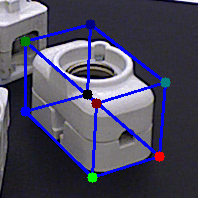
\includegraphics[width=0.45\linewidth]{bb8}
    	\caption{The control points of the object's bounding box.}
	\end{subfigure}
	\hfill
	\begin{subfigure}[b]{0.45\textwidth}
		\centering
    	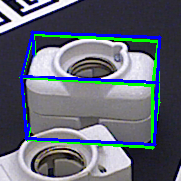
\includegraphics[width=0.45\linewidth]{bb8_prediction}
    	\caption{The final estimated pose. Green is the groundtruth.}
	\end{subfigure}
	\caption{Example images displaying the functioning of BB8. Images taken from \cite{bb8}.}
\end{figure}
Despite its differences to \cite{brachmann1}, the object's position is not predicted directly either, but instead regressed by solving the perspective-n-point (PnP) problem of the correspondences of the corners of the object's bounding box and the projected 2D locations of the corners predicted by the network. The architecture of the first and second net is based on VGG respectively but with the last layer cut off and replaced by a fully connected layer which is fine-tuned. 
\nnewline
The first network, which segments the image, helps estimating the pose of the object in a way that the second network positions its window at the center of the segmentation and predicts the pose. The pose prediction works by estimating the 2D locations of the 3D corners of the object's bounding box. The network reasons globally about the object by not moving the window containing the object during training and prediction. The authors argue that patch-based pose estimators are typically very noisy, and hence require a robust optimization scheme, like RANSAC. 
\nnewline
Unfortunately, BB8's take on pose estimation fails on symmetric objects, when implemented directly as described above. To address this problem, the authors first estimate the rotational angle of the object, and mirror the image if necessary. This way, a CNN can be trained only on a certain range of the angle of the pose.
\nnewline
The proposed method offers good performance and can compete with and partly surpasses state-of-the-art research. Yet, object coordinates provide high accuracy too and due to the assumption of the author of this work, that the often merely patch-wise visibility of the surgical instruments calls for a non-global reasoning design BB8 is followed any further in this work.

\paragraph{SSD-6D.}

The system carved out by \cite{ssd-6d} is based on the work by \cite{ssd} dubbed Single-Shot Multibox Detector, or short SSD. Their take on 6D pose estimation is especially alluring, as the authors train the network exclusively on synthetic data. Good results would imply that the lack of large already annotated datasets for 6D pose estimation in the field of biomedical imaging could be overcome by simply generating the desired amount of data and training the network on this artificial data. 
\nnewline
In contrast to BB8 and Brachmann et al., who both rather inferred what part of the image corresponds to what of the object to be detected, Kehl et al. let the network estimate the probability of a discrete viewpoint, which is essentially a view of a camera on the object. Those viewpoints are sampled equidistant alongside a degree step-size to represent all possible poses of the objects. According to the authors, the number of views that are necessary to produce good results is 642. In addition, in-plane rotations of the objects are sampled as well. This view estimate combined with an estimate on the rotation is used to generate pose predictions. 
\nnewline
\begin{figure}[!tbp]
	\centering
	\begin{subfigure}[b]{0.3\textwidth}
		\centering
    	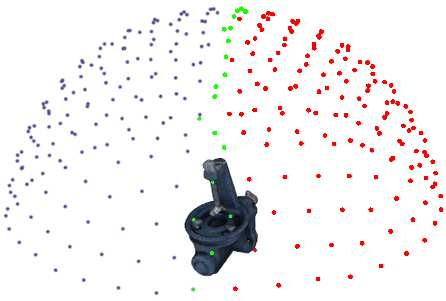
\includegraphics[width=\linewidth]{ssd_6d_sphere}
    	\caption{An exampe of a discrete distribution of viewpoints on an object.}
	\end{subfigure}
	\hfill
	\begin{subfigure}[b]{0.6\textwidth}
		\centering
    	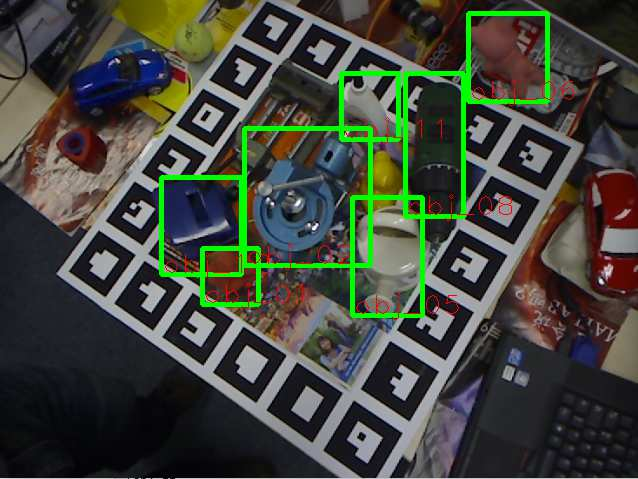
\includegraphics[width=0.45\linewidth]{ssd_6d_bb}
    	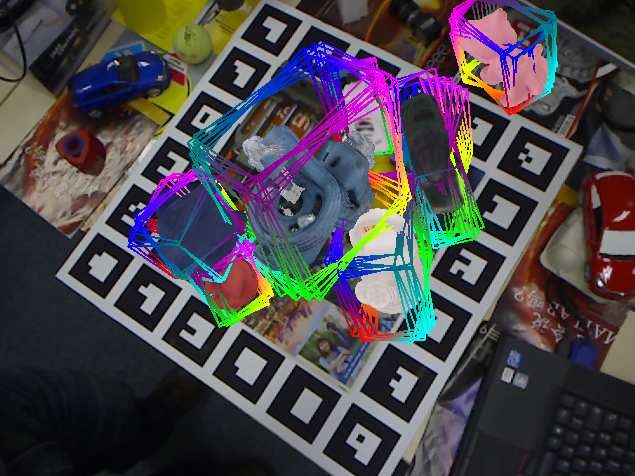
\includegraphics[width=0.45\linewidth]{ssd_6d_pose}
    	\caption{Left image: An example for bounding boxes found by the SSD-6D network. Right image: The most confident views and rotations for those boxes.}
	\end{subfigure}
	\caption{Example images displaying the functioning of SSD-6D. Images taken from \cite{ssd-6d}}
\end{figure}
The network architecture, that is inspired by SSD, produces feature maps using branches from a pre-trained Inception V4, which was introduced in \cite{inceptionv4}. The branches are kernels of different size and the resulting maps are again convolved with kernels that predict the object class, 2D bounding box, viewpoint scores and in-plane rotations. A non-max suppression then selects only the strongest candidates. The network is trained entirely on images from the MS COCO dataset \cite{mscoco} that the authors rendered the objects into with random transformations, i.e. the whole training set is generated. For each transformation, the network is given the closest discrete viewpoint, in-plane rotation and the tightest bounding box as a regression target. As an optimization target during error-back propagation, the authors employ a loss similar to the one of SSD \cite{ssd} or YOLO \cite{yolo}. 
\nnewline
Like stated above, the actual 6D pose estimation task is solved by using the viewpoint, the bounding box and the in-plane rotation. The author's reasoning, that their approach on pose estimation is a more natural one than pose regression makes sense, as for example a human being rather learns what an object looks like from different angles than regression of object coordinates. Nevertheless, the network produces rather bad results if not the last step of optimization is applied. That is, after obtaining an initial pose from the network, an optimization scheme extracts 3D contour points from the rendered hypothesis, which are then used to find the closest edges to minimize a projection error and improve the overall pose. 
\nnewline
What can be easily verified is that the first estimate of the 6D pose is rather bad. Compared with other works, which directly produce good results with the method as is, here the most important part seems to be the second optimization program. But then, this optimization could also be used in \cite{brachmann2} or \cite{bb8} as a last step, making it a good contribution but as an addition. Thus the network architecture isn't considered any further.

\paragraph{Kurmann et al.}

Despite the obvious field for 6D pose estimation being autonomous robots interacting with their environment, there exists work that directly work on pose estimation of surgical instruments in minimally invasive surgery, for example \cite{kurmann}. The authors of that paper argue that the common two-stage pipeline for 6D pose estimation, that consists of object detection and then the actual pose estimation, is rather sensitive to parameter-tuning and results in a more complicated design. They also criticize that a sliding window approach might miss very small or very large instruments. 
\nnewline
Similarly to object coordinate regression, Kurmann et al. develop a system that produces probabilities of the presence of an object but not in a dense way but instead only for the joints of the tools. Their design draws on a scene model which holds how many tools can be visible at most, what tools are currently visible and what parts of those tools. 
\nnewline
The architecture of the employed network is based on the U-Net of \cite{oronneberger} and trained by optimizing the cross-entropy derived from the scene model described earlier. To adapt the architecture of U-Net, which stems from semantic segmentation, a new fully-connected layer, which is directly connected with the first layer of the network, is introduced and trained to predict probabilities of the different instruments. 
\nnewline
The results of the design look promising and runtimes per image are around $100 ms$, enabling it to be deployed as a near-realtime solution. On the other hand it seems like mainly literature of the biomedical imaging was considered and compared, i.e. overlooking the vast literature on 6D pose estimation in other fields. This and because object coordinates is a well-researched approach, the latter was chosen as a basis for this work over the one in \cite{kurmann}. 

\subsection{Learning-Based: Object Coordinate Regression}

An interesting section of learning-based pose estimation are the works employing the method of so-called object coordinate regression (see Section \ref{objectcoordinates}). The idea is based on \cite{tsharp} and \cite{firstcoordinateregression}. The first used it to estimate the pose of a human body, the latter to regress the cameras position in a scene retrieved from a single RGB-D image.
\nnewline
\cite{brachmann1} achieved record-breaking results on 6D pose estimation for texture-less objects and good performance in general and thus spawned more research in this direction. Brachmann et al. based their work not on trees but whole forests instead to regress the object's pose. The forests are trained to jointly predict the probability of object instances as well as the object coordinate probability for a given pixel, i.e. the leaves represent probability distributions. The energy function that processes the output of the forest imposes an energy minimization problem to regress the object's pose. To improve the resulting pose and make the design more robust to outliers, a RANSAC-like scheme is proposed that iteratively samples pose hypotheses and finally outputs the pose with the lowest energy.
\nnewline
In \cite{brachmann2}, Brachmann et al. adjusted their pipeline from \cite{brachmann1} to work with RGB-only images. To reduce uncertainty in the object instance and coordinate predictions they incorporate a self-developed auto-context framework and also marginalize the object coordinates over the depth information to cope with the missing fourth channel. The proposed system outperforms Brachmann's previous work but still relies on decision trees. 
\nnewline
\cite{akrull} elaborated \cite{brachmann1} by replacing the energy function by a CNN. This way they were able to further improve the performance of the already powerful system and, more importantly, transfer object coordinate regresion to modern deep neural networks. \cite{poseagent} develops a novel synergy between the already known regression forest and a CNN which resembles the actual PoseAgent. The CNN is reponsible to predict the best pose taking into account the output of the forest. Brachmann et al. are able to achieve state-of-the-art results and improve resource utilization. Although \cite{trees-vs-cnn} finds, that random forests partly offer a slightly superior performance, their accuracy can still be comparable and we are still only on the verge of what is possible with neural networks.

\paragraph{Pertsch.}

Although \cite{pertsch} also works with RGB-D images, we present his work here as the author proposes an easy extension to adapt the entire process to RGB-only images and presents promising results. The work by Pertsch is based on \cite{brachmann1}, i.e. likewise uses object coordinates  (see section \ref{objectcoordinates}), but replaces the random forest with a CNN. The developed pose estimation pipeline relies on three steps. The first one segments the image, the second regresses the object coordinates, and the last one evaluates pose hypotheses. 
\nnewline
We don't to go into detail into the first operation of the pipeline as our training and test data already includes segmentations and we can hence omit it completely. The purpose of the segmentation masks produced in the first step is to crop the area that the CNN of the second stage has to evaluate and also to calculate the score of a pose hypothesis in the energy function of the last stage. 
\nnewline
The second stage, which is more interesting for us, uses a multilayer CNN-architecture to predict the object coordinates. The architecture resembles an encoder-decoder network with fully-connected layers in the middle. This supposedly enables the network to detect features of the input images on a global scale as the perceptive fields of the fully-connected neurons is effectively enlarged to the full input dimensions, whereas a fully-convolutional network might miss certain connections. 
\nnewline
Inspired by \cite{oronneberger}, the author assimilates skip-layer connections. The network computes object coordinates for each pixel of the cropped image. To train the network the groundtruth is computed by rendering the model of the 3D object using the manually annotated groundtruth pose. Since the prediction of the object coordinates is typically quite noisy \cite{bb8}, \cite{pertsch} employs a RANSAC-scheme to improve the quality of the predicted final pose. Two different methods to retrieve the pose are presented in the work, one relying on the energy function introduced in \cite{brachmann1} but in an altered version taking into account the binary segmentation mask opposed to the random forest probabilities, and one procedure solely drawing on RGB information without the additional groundtruth depth of a sensor. The latter, which is more relevant for us as we do not have any depth readings, is based on the earlier presented \cite{brachmann2}. 
\nnewline
Instead of penalizing depth divergences, the number of pixels whose reprojection error is greater than a certain threshold is minimized iteratively by the RANSAC algorithm. This allows for the RGB-only extension that the author proposes but does not elaborate any further beyond a short passage. The fourth dimension is discarded by substituting the Kabsch algorithm that regresses a set of 3D-3D point pairs with a PnP solver, which takes at least four 3D-2D point correspondences as input and calculates the implied pose. The 3D reprojection error is replaced by the 2D reprojection error, due to the lack of a groundtruth point cloud. We pursue a similar approach in our work which differs in architecture in the network, the steps of the pipeline (i.e. only object coordinate prediction and pose estimation) and the input data. But the general ideas of \cite{pertsch} and especially \cite{brachmann1} are adopted and further complemented with current research and active and incremental learning.

\section{Research on Active and Online Learning}

Online learning considers how to incorporate new available data into the model or neural network and active learning is the field of selecting data that a human should annotate manually, because the model does not perform as well on it. The literature survey\cite{activesurvey} gives an overview over methods developed before 2011. Wang and Shang, the authors of \cite{dwang}, might be among the first to incorporate active learning into deep learning though, according to \cite{zhou}. In \cite{hyperspectral}, Al Rahhal et al. apply a similar idea to hyperspectral image classification, a task that shares the foibles to be tedious and time-consuming with biomedical image annotation. The authors developed an active selection paradigm to electrocardiogram classification. 

\paragraph{Zhou et al.}

In \cite{zhou}, Zhou et al. describe a novel process of actively demanding data to be annotated to improve the network quality and apply the newly available data in an incremental manner. They focus on this area because annotating biomedical images is still a time-consuming task that requires a lot of expertise and skill.
\nnewline
Opposed to retraining from scratch, the network is fine-tuned by an incremental tuning algorithm. According to the authors, researchers have shown that this offers superior performance. In contrast to our task, the authors want to achieve improvements on image classification and frame detection, but work on biomedical images nonetheless.
\nnewline
\begin{figure}[!tbp]
	\centering
    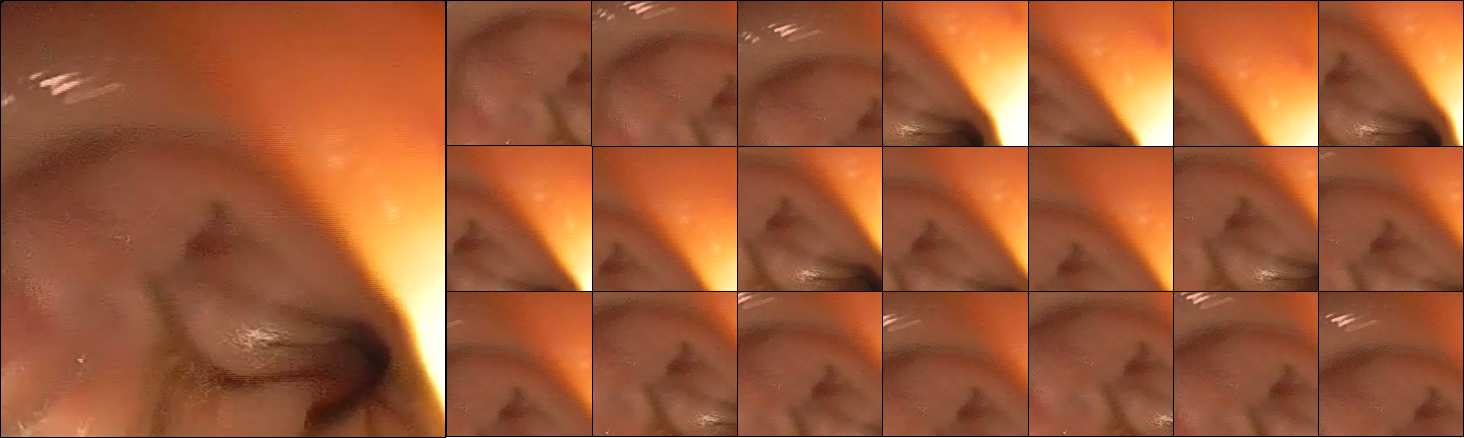
\includegraphics[width=0.7\linewidth]{fine_tuning}
	\caption{A candidate (left) and the patches generated sharing the same label. \cite{zhou}}
	\label{fig:zhou}
\end{figure}
The authors state that computer-aided-diagnosis (CAD) systems usually provide a candidate generator, which can quickly produce candidates, including true and false positives, to train classifiers with. The goal is to eleminate as many false positives as possible, while keeping the true ones. Through data augmentation the learner can be made more robust to unforeseen situations. For this, numerous patches sharing the same label are generated from the candidate, as can be seen in Figure \ref{fig:zhou}. 
\nnewline
The active selection process of candidates requires a measure of the worthiness of a candidate. To achieve this, the entropy and diversity of patches are calculated using the network's predictions for the patches of a candidate. Entropy is calculated as the sum of the negative log-likelihood, whereas diversity captures the summed up differences of the probability values, that the network produces for the patches of a specific candidate and label. Intuitively, for a candidate the entropy of all its patches should be high, as the neural network should be sure of a prediction, and the diversity low, as the patches are generated from the same candidate and should share the same label. Candidates with contradicting patches or low entropy can then be selected for manual annotation.
\nnewline
The procedure produces good results of 95\% correctly labeled images while using only 5\% of the available dataset for training. Learning from scratch or random selection of next candidates are quickly surpassed in terms of accuracy. The presented method needs around 4 manually annotated candidates to achieve the accuracy of the random process at 18 or learning from scratch at 22 manually annotated candidates.
\nnewline
In our case, data augmentation is possible, as we can render synthetic images, but the unnatural lightning and shadowing might decrease the accuracy of the design. The question of how to find  a worthiness measure arises when projecting Zhou et al.'s approach to pose estimation, as we can't directly tell how sure a network is when predicting a pose. But it provides a good direction of how to approach active learning.

\paragraph{Liu \& Ferrari.}

\begin{figure}[!tbp]
	\centering
    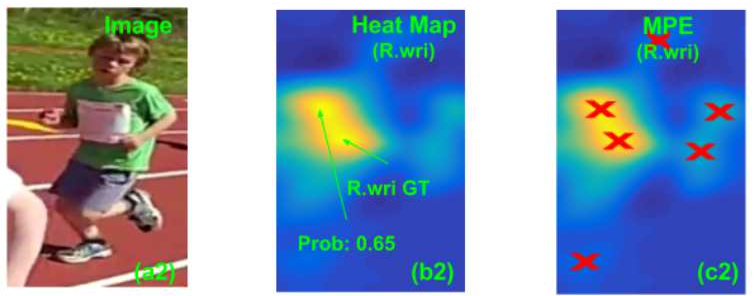
\includegraphics[width=0.6\linewidth]{human_pose_heatmap}
    \caption{An image of a human body, the corresponding heatmap as well as the result of the Multiple Peak Entropy (MPE). \cite{humanpose}}
    \label{fig:humanpose}
\end{figure}
In \cite{humanpose}, Liu and Ferrari describe new strategy for active learning for human pose estimation, a time-consuming task to produce groundtruth annotations for. Their key contributions consist of an uncertainty estimator for the joint predictions produced by a Convolutional Pose Machine (CPM), and an annotation interface that reduces the time needed by a human annotator to click joints.
\nnewline
The active learning scheme incorporates influence and uncertainty cues. Influence cues account for the property that images that are similar to other unlabeled images could propagate information, and thus provide a higher information gain. The uncertainty cues on the other hand are measured by the uncertainty estimator. The estimator considers all locally optimal predictions of the CPM. This way, a joint prediction that contains multiple weak peaks, i.e. is a rather uncertain prediction, can be selected for manual annotation. Liu and Ferrari called this criterion the Multiple Peak Entropy (MPE), whose way of functioning can be seen in Fig. \ref{fig:humanpose}. The final selection process then takes both cues into account when requesting an image to be manually annotated.
\nnewline
In addition to this active learning mechanism, an innovative joint annotation interface is proposed that reduces the annotation time significantly. The system generates a hypothesis for the joint locations and presents it to the user, while segmenting the image into non-overlapping areas. Instead of having to precisely click a pixel the human annotator then simply right-clicks the area around the joint, if marked location is already correct. If not, a left click on the exact position is necessary. It is easy to see, that this new option does not lengthen the annotation procedure, but, au contraire, can speed it up.
\nnewline
The results of \cite{humanpose} look auspicious, as a reduction in annotation time can be achieved through the introduced interface, and an increase in precision through the active learning method. Regrettably, it cannot be directly applied to our problem, as we need a problem-specific certainty estimator. But the idea of requesting similar images to be annotated might yield a performance gain. Similarly to the presented interface, we present the user with an initial probable pose, too, to make only small corrections necessary.